\section{系统调用}

在初版NPUcore中,我们实现了系统调用81个,并满分通过了libc测试。如今,我们在NPUcore-IMPACT中已经增加到90个POSIX系统调用(如图\ref{fig:syscall1}和\ref{fig:syscall2}),完整版可参考“os/src/arc/la64/syscall_id.rs”。
\begin{figure}[htp]
    \centering
    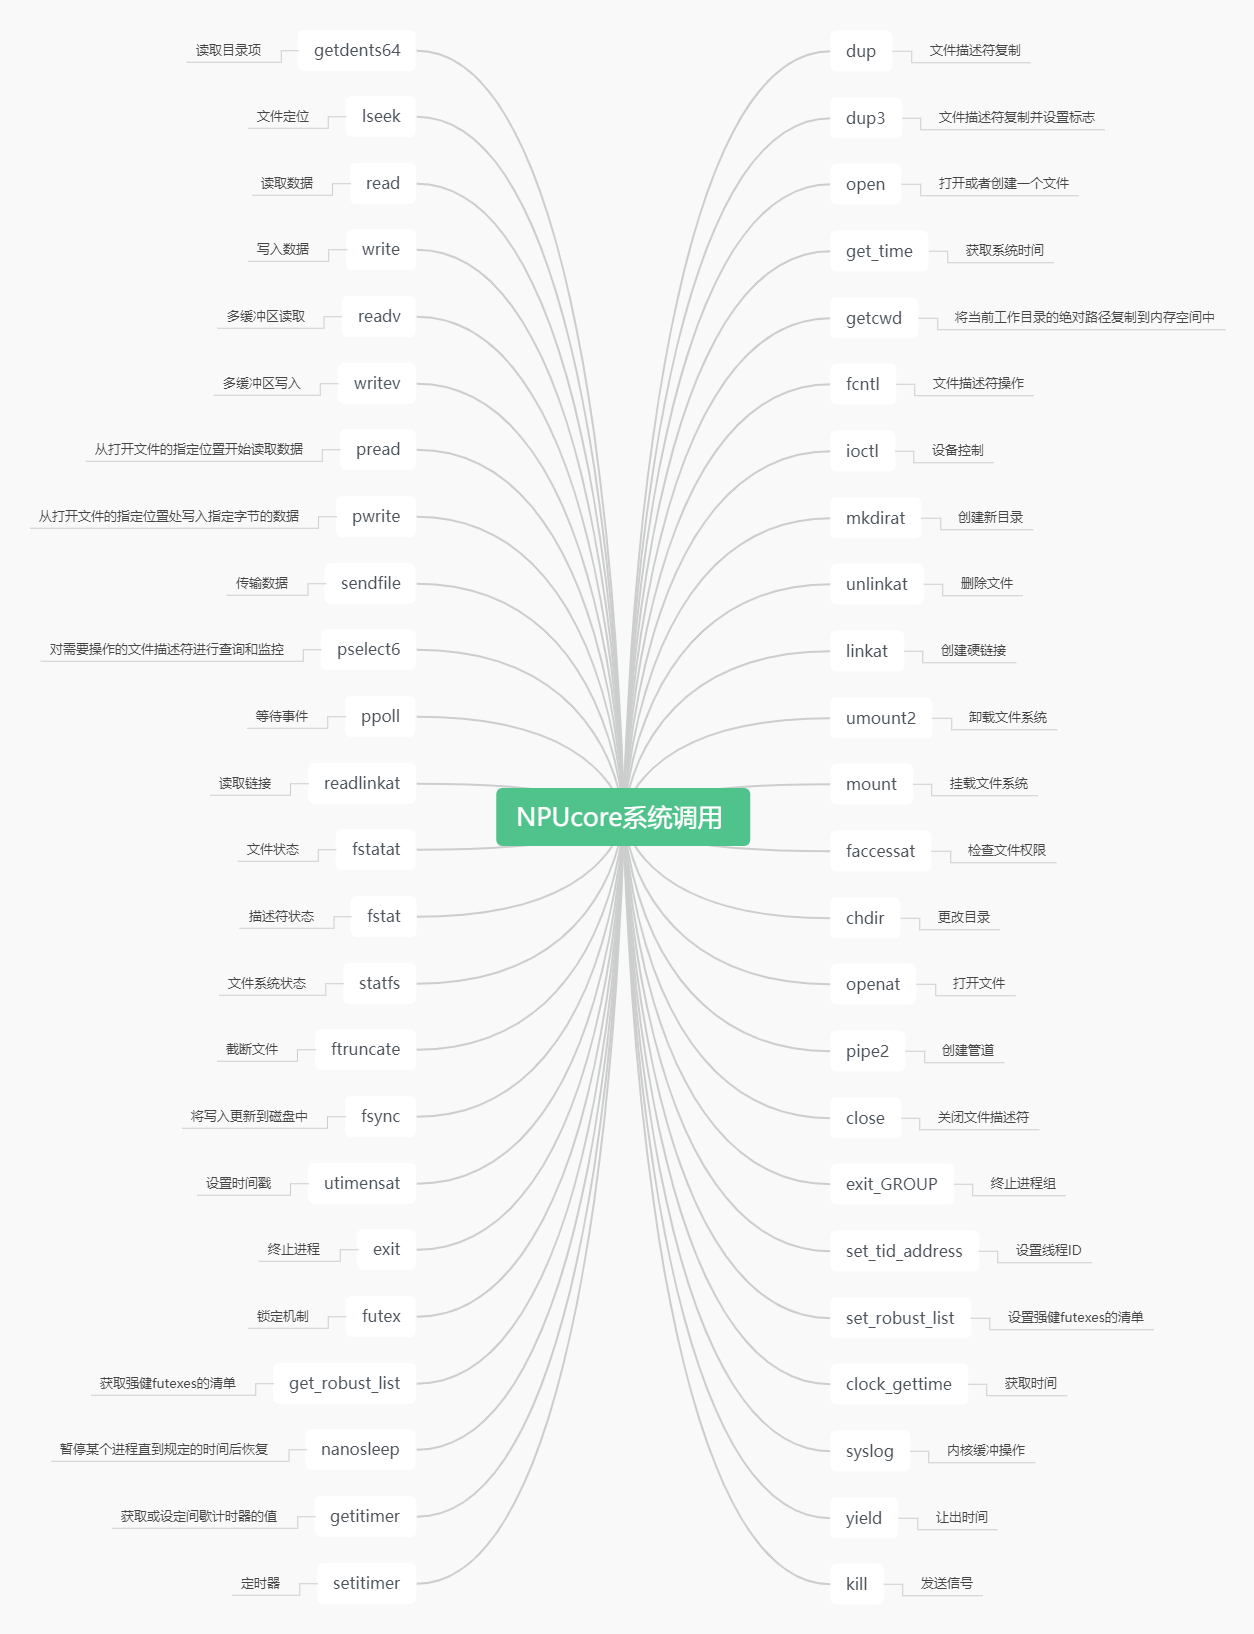
\includegraphics[width=1\linewidth]{figs/01-03-NPUcore系统调用1.png}
    \caption{NPUcore-IMPACT系统调用(其一)}
    \label{fig:syscall1}
\end{figure}

\begin{figure}[htp]
    \centering
    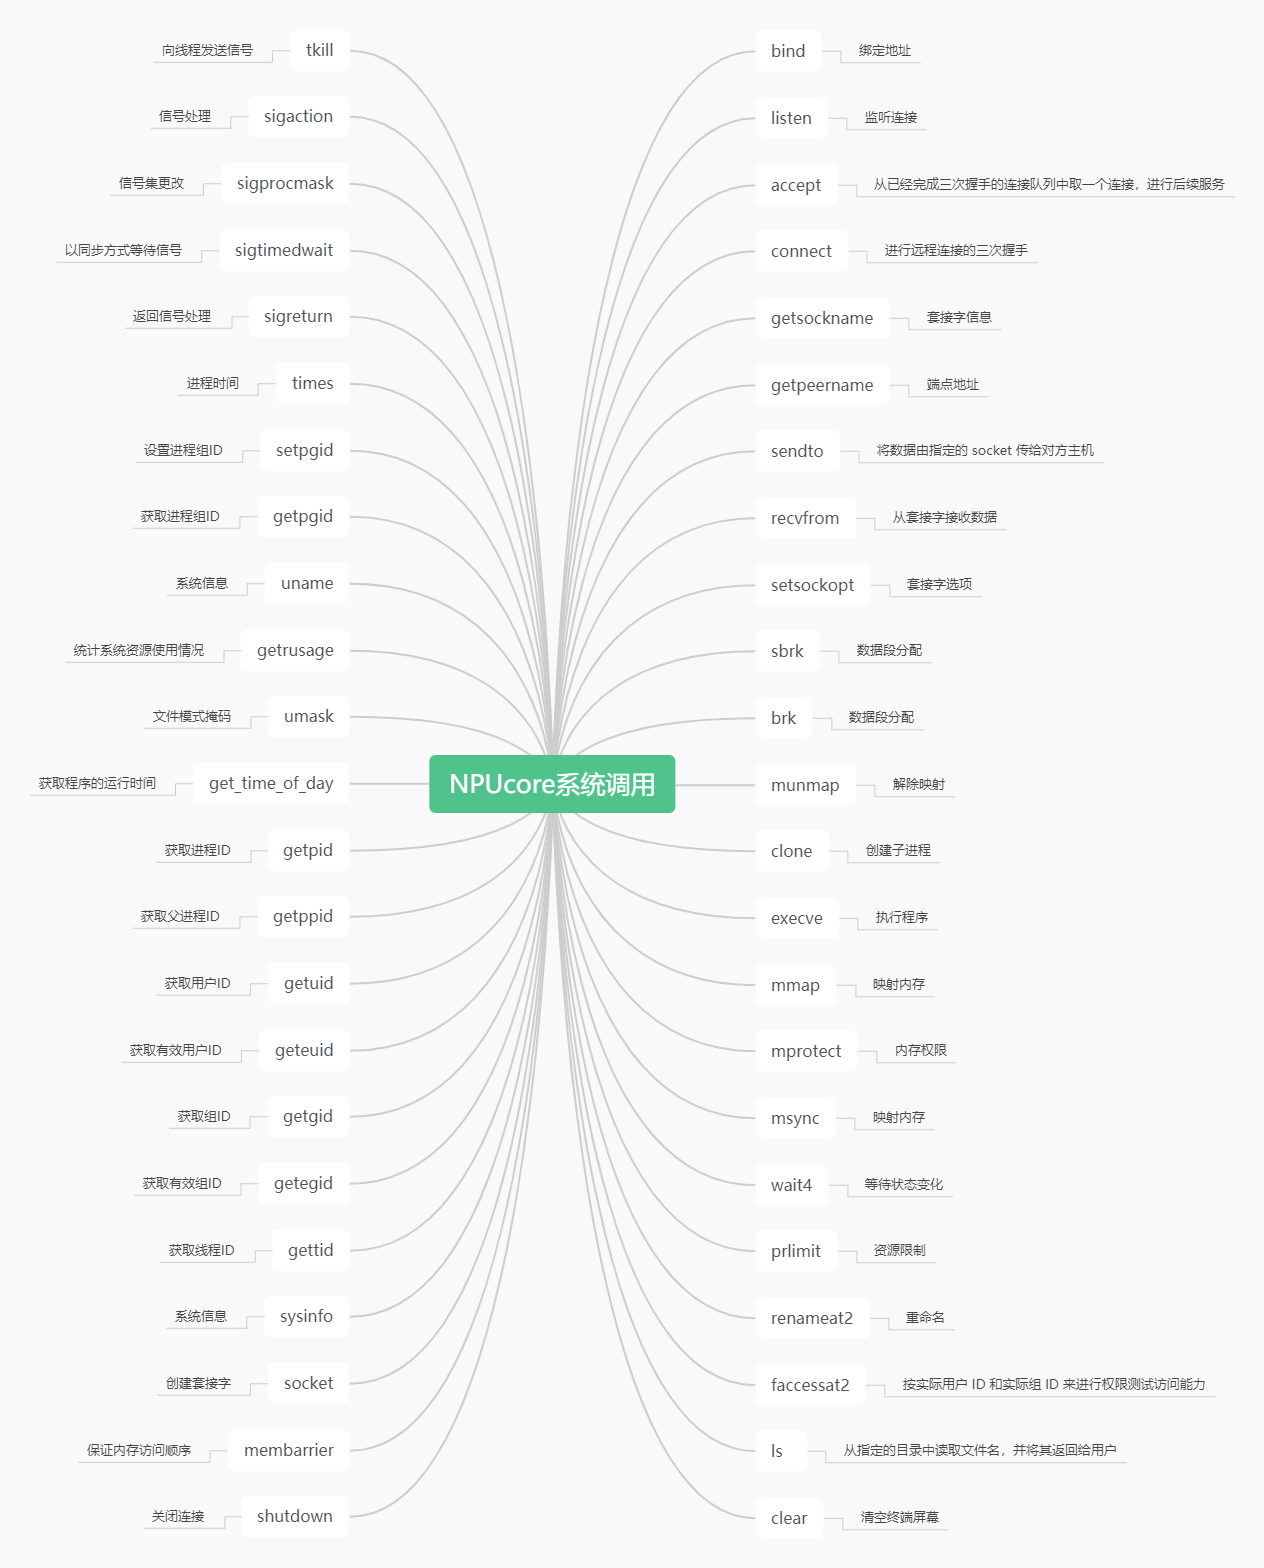
\includegraphics[width=1\linewidth]{figs/01-03-NPUcore系统调用2.png}
    \caption{NPUcore-IMPACT系统调用(其二)}
    \label{fig:syscall2}
\end{figure}

\section{NPUcore-IMPACT目录树}

\begin{lstlisting}[language={bash}, label={code:content},
	caption={目录树}]
    ./
    |-- Makefile            // 根目录makefile,用于链接到os目录
    |-- README.md           // Readme
    |-- dependency          // 使用的外部包
    |   |-- ext4            // EXT4文件系统(初赛不提交该版本)
    |   |-- virtio-drivers  // 虚拟设备
    |-- os                  // OS内核
    |   |-- Cargo.lock
    |   |-- Cargo.toml
    |   |-- Makefile        // 核心makefile
    |   |-- buildfs.sh      // 建立fat32文件系统
    |   |-- cpio.log
    |   |-- la_fat          // fat32文件系统脚本
    |   |-- src             // 核心代码
    |   |   |-- arch        // LA2K1000底层交互
    |   |   |   |-- la64
    |   |   |   |   |-- board
    |   |   |   |   |   |-- 2k1000.rs
    |   |   |   |   |-- config.rs
    |   |   |   |   |-- entry.asm
    |   |   |   |   |-- kern_stack.rs
    |   |   |   |   |-- la_libc_import.rs
    |   |   |   |   |-- laflex.rs
    |   |   |   |   |-- load_img.S
    |   |   |   |   |-- mod.rs
    |   |   |   |   |-- register
    |   |   |   |   |   |-- base
    |   |   |   |   |   |-- macros.rs
    |   |   |   |   |   |-- mmu
    |   |   |   |   |   |-- mod.rs
    |   |   |   |   |   |-- ras
    |   |   |   |   |   |-- timer
    |   |   |   |   |-- sbi.rs
    |   |   |   |   |-- switch.S
    |   |   |   |   |-- switch.rs
    |   |   |   |   |-- syscall_id.rs
    |   |   |   |   |-- time.rs
    |   |   |   |   |-- tlb.rs
    |   |   |   |   |-- trap
    |   |   |   |       |-- context.rs
    |   |   |   |       |-- mem_access.rs
    |   |   |   |       |-- mod.rs
    |   |   |   |       |-- trap.S
    |   |   |   |-- mod.rs
    |   |   |-- console.rs
    |   |   |-- drivers     // 设备块
    |   |   |   |-- block
    |   |   |   |   |-- block_dev.rs
    |   |   |   |   |-- mem_blk.rs
    |   |   |   |   |-- mod.rs
    |   |   |   |   |-- virtio_blk.rs
    |   |   |   |-- mod.rs
    |   |   |   |-- serial
    |   |   |       |-- mod.rs
    |   |   |       |-- ns16550a.rs
    |   |   |-- fs          //文件系统
    |   |   |   |-- cache.rs
    |   |   |   |-- dev
    |   |   |   |   |-- hwclock.rs
    |   |   |   |   |-- mod.rs
    |   |   |   |   |-- null.rs
    |   |   |   |   |-- pipe.rs
    |   |   |   |   |-- socket.rs
    |   |   |   |   |-- tty.rs
    |   |   |   |   |-- zero.rs
    |   |   |   |-- directory_tree.rs
    |   |   |   |-- fat32
    |   |   |   |   |-- bitmap.rs
    |   |   |   |   |-- dir_iter.rs
    |   |   |   |   |-- efs.rs
    |   |   |   |   |-- inode.rs
    |   |   |   |   |-- layout.rs
    |   |   |   |   |-- mod.rs
    |   |   |   |   |-- vfs.rs
    |   |   |   |-- file_trait.rs
    |   |   |   |-- filesystem.rs
    |   |   |   |-- layout.rs
    |   |   |   |-- mod.rs
    |   |   |   |-- poll.rs
    |   |   |   |-- swap.rs
    |   |   |-- lang_items.rs
    |   |   |-- linker.in.ld
    |   |   |-- main.rs
    |   |   |-- mm          // 访存
    |   |   |   |-- address.rs
    |   |   |   |-- frame_allocator.rs
    |   |   |   |-- heap_allocator.rs
    |   |   |   |-- map_area.rs
    |   |   |   |-- memory_set.rs
    |   |   |   |-- mod.rs
    |   |   |   |-- page_table.rs
    |   |   |   |-- zram.rs
    |   |   |-- syscall     // 系统调用
    |   |   |   |-- errno.rs
    |   |   |   |-- fs.rs
    |   |   |   |-- mod.rs
    |   |   |   |-- process.rs
    |   |   |   |-- socket.rs
    |   |   |-- task        // 线程
    |   |   |   |-- context.rs
    |   |   |   |-- elf.rs
    |   |   |   |-- manager.rs
    |   |   |   |-- mod.rs
    |   |   |   |-- pid.rs
    |   |   |   |-- processor.rs
    |   |   |   |-- signal.rs
    |   |   |   |-- task.rs
    |   |   |   |-- threads.rs
    |   |   |-- timer.rs
    |   |-- vendor          // 大赛要求的离线包
    |-- user                // user测例与用户系统调用
    |   |-- Cargo.lock
    |   |-- Cargo.toml
    |   |-- Makefile
    |   |-- busybox_lua_testsuites
    |   |-- loongarch64
    |   |-- src
    |   |   |-- bin
    |   |   |-- console.rs
    |   |   |-- la_libc_import.rs
    |   |   |-- lang_items.rs
    |   |   |-- lib.rs
    |   |   |-- linker-2k500.ld
    |   |   |-- linker.ld
    |   |   |-- syscall.S
    |   |   |-- syscall.rs
    |   |   |-- usr_call.rs
    |   |-- user_C_program
    |-- util                // 大赛官方qemu与镜像生成
        |-- mkimage
        |-- qemu
    
\end{lstlisting}